% Format teze zasnovan je na paketu memoir
% http://tug.ctan.org/macros/latex/contrib/memoir/memman.pdf ili
% http://texdoc.net/texmf-dist/doc/latex/memoir/memman.pdf
% 
% Prilikom zadavanja klase memoir, navedenim opcijama se podešava 
% veličina slova (12pt) i jednostrano štampanje (oneside).
% Ove parametre možete menjati samo ako pravite nezvanične verzije
% mastera za privatnu upotrebu (na primer, u b5 varijanti ima smisla 
% smanjiti 
\documentclass[12pt,oneside]{memoir}

% Paket koji definiše sve specifičnosti mastera Matematičkog fakulteta
\usepackage[latinica]{matfmaster}
%
% Podrazumevano pismo je ćirilica.
%   Ako koristite pdflatex, a ne xetex, sav latinički tekst na srpskom jeziku
%   treba biti okružen sa \lat{...} ili \begin{latinica}...\end{latinica}.
%
% Opicija [latinica]:
%   ako želite da pišete latiniciom, dodajte opciju "latinica" tj.
%   prethodni paket uključite pomoću: \usepackage[latinica]{matfmaster}.
%   Ako koristite pdflatex, a ne xetex, sav ćirilički tekst treba biti
%   okružen sa \cir{...} ili \begin{cirilica}...\end{cirilica}.
%
% Opcija [biblatex]:
%   ako želite da koristite reference na više jezika i umesto paketa
%   bibtex da koristite BibLaTeX/Biber, dodajte opciju "biblatex" tj.
%   prethodni paket uključite pomoću: \usepackage[biblatex]{matfmaster}
%
% Opcija [b5paper]:
%   ako želite da napravite verziju teze u manjem (b5) formatu, navedite
%   opciju "b5paper", tj. prethodni paket uključite pomoću: 
%   \usepackage[b5paper]{matfmaster}. Tada ima smisla razmisliti o promeni
%   veličine slova (izmenom opcije 12pt na 11pt u \documentclass{memoir}).
%
% Naravno, opcije je moguće kombinovati.
% Npr. \usepackage[b5paper,biblatex]{matfmaster}

% Pomoćni paket koji generiše nasumičan tekst u kojem se javljaju sva slova
% azbuke (nema potrebe koristiti ovo u pravim disertacijama)
\usepackage{pangrami}

% Paket koji obezbeđuje ispravni prikaz ćiriličkih italik slova kada
% se koristi pdflatex. Zakomentarisati ako na sistemu koji koristite ovaj
% paket nije dostupan ili ako ne radi ispravno.
\usepackage{cmsrb}

% Ostali paketi koji se koriste u dokumentu
\usepackage{listings} % listing programskog koda

% Datoteka sa literaturom u BibTex tj. BibLaTeX/Biber formatu
\bib{matfmaster-primer}

% Ime kandidata na srpskom jeziku (u odabranom pismu)
\autor{Luka B. Đorović}
% Naslov teze na srpskom jeziku (u odabranom pismu)
\naslov{Analiza slučajeva upotrebe relacionih i kolonski orijentisanih nerelacionih baza podataka}
% Godina u kojoj je teza predana komisiji
\godina{2024}
% Ime i afilijacija mentora (u odabranom pismu)
\mentor{др Saša \textsc{Malkov}, vandredni profesor\\ Универзитет у Београду, Математички факултет}
% Ime i afilijacija prvog člana komisije (u odabranom pismu)
\komisijaA{др Ана \textsc{Анић}, ванредни професор\\ University of Disneyland, Недођија}
% Ime i afilijacija drugog člana komisije (u odabranom pismu)
\komisijaB{др Лаза \textsc{Лазић}, доцент\\ Универзитет у Београду, Математички факултет}
% Ime i afilijacija trećeg člana komisije (opciono)
% \komisijaC{}
% Ime i afilijacija četvrtog člana komisije (opciono)
% \komisijaD{}
% Datum odbrane (obrisati ili iskomentarisati narednu liniju ako datum odbrane nije poznat)
\datumodbrane{15. јануар 2016.}

% Apstrakt na srpskom jeziku (u odabranom pismu)
\apstr{}

% Ključne reči na srpskom jeziku (u odabranom pismu)
\kljucnereci{анализа, геометрија, алгебра, логика, рачунарство, астрономија}

\begin{document}
% ==============================================================================
% Uvodni deo teze
\frontmatter
% ==============================================================================
% Naslovna strana
\naslovna
% Strana sa podacima o mentoru i članovima komisije
\komisija
% Strana sa posvetom (u odabranom pismu)
\posveta{Ovaj rad posvećujem...}
% Strana sa podacima o disertaciji na srpskom jeziku
\apstrakt
% Sadržaj teze
\tableofcontents*

% ==============================================================================
% Glavni deo teze
\mainmatter
% ==============================================================================

% ------------------------------------------------------------------------------
\chapter{Uvod}
% ------------------------------------------------------------------------------

Podaci su najstabilniji deo svakog sistema. Oni su reprezentacija činjenica, koncepata jednog sistema kao i instrukcija u formalizovanom stanju spremnom za dalju interakciju, interpretaciju ili obradu od strane korisnika ili mašine. Iako kroz svoju istoriju računatstvo važi za oblast koja uvodi nove tehnologije i alate neverovatnom brzinom to  nije slučaj za svaku njenu granu. Postoje oblasti koje se kroz istoriju nisu menjali, ili su se slabo menjali i proširivali. Primera za to ima puno i oni su uglavnom usko vezani za funkcionalne principe koji se prožimaju kroz računarske mreže, kompilatore, operativne sisteme, sisteme za upravljanje podacima itd. 

Kada je reč o istoriji sistema za upravljanje podacima, izdvojio bih tri glavne faze: vreme pre relacionih sistema, vreme neprikosnovene vladavine relacionih sistema i nastanak alternativa relacionim sistemima pod grupnim nazivom NoSQL.

Do 70ih i nastanka relacionih sistema za upravljanje podacima, rukovanje podacima izvodilo se kroz pisanje i čitanje sa fajl sistema operativnog sistema. Rukovanje većim količinama podataka nije bilo standardizovano ni na koji način već su se konvencije uvodile na nivou organizacija. Apolo sletanje na Mesec realizovano je koristeći ovakav vid rada sa podacima, što ovaj poduhvat čini utoliko neverovatnim. 

S obzirom da je ovaj vid rada sa podacima imao mnogbrojne mane, među kojima je jedan od glavnih bio težak pristup podacima, javile su se potrebe za unapređenjem. Najuspešniji je bio Edgar F. Codd \footnote{Edgar Frank "Ted" Codd (19 Avugst 1923 – 18 April 2003) Američki računarski naučnik }  koji je 1970. godine objavio rad pod imenom "A Relational Model of Data for Large Shared Data Banks" kao rezultat istraživanja i sopstvenih teorija o organizaciji podataka.  Kao dokaz da je njegov model moguće implementirati pokrenut je System R, čiji je rezultat bio i pojava SQL-a (Structured Query Language) kao standardizovanog jezika za rad sa podacima. Nakon toga pojavili su se Oracle i IBM sa svojim komercijalnim proizvodima za upravljanje relacionih baza podataka. Naredni period obeležio je rad sa podacima koristecći relacioni model.  

XXI vek doneo je sa sobom ubrzanu digitalizaciju, povećanu dostpunost interneta, samim tim pojavila se potreba za obradom veće količine podataka. Sve ovo je pokazalo pojedine slabosti dosadašnjih sistema zasnovane na relacionim modelima, koji nisu mogli u svim segmentima da odgovore na zahteve modernog doba. Ovi problemi obično su poznati pod gruonim imenom "problemi velikih podataka" (BigData problems). Došlo je do pojave niza novih modela i principa za čuvanje podataka, a svi pod grupnim imenom "NoSQL" (ili nerelacione) baze podataka.
Sistematizovanje ogromne količine fizičkog prostora na disku na kojem se podaci mogu čuvati i kasnije koristiti, kao i fleksibilnost strukture podataka sa kojima se radi , jesu glavni aktuelni problemi tog vremena na koje su se fokusirale tehnologije nastale u NoSQL pokretu.
Decenije vladavine  relacionih sistema za čuvanje podataka ostavile su dubok trag u praksama rada sa podacima, i sa razlogom predstavljaju defakto standard i dan danas, te je zaočekivati postojanje doze skepse pri korišćenju tehnologija nastalih u ovoj fazi. 

Kao važna grupa nerelacionih izdvajaju se kolonski-orijentisane baze podataka. One su uvele tada nekonvencionalne koncepte čuvanja podataka po kolonama. Dakle fizički na disku skladištile su se vrednosti jedne kolone jedna do druge, sa referencom na red kojem pripadaju. To sa sobom vuče razne mogućnosti za optimizaciju ali i novih pristupa modelovanja i organizacije podataka. Ovakav način skladištenja ispitavan je još davnih 70ih godina XX veka, međutim u ranim godinama XXI veka došlo je do obnove interesovanja u akademskim ali i industrijskim krugovima. 

Nijedan od navedenih koncepata nije univerzalno rešenje, zato je bitno postojanje materijala koji se bave analizom slučajeva upotrebe tih tehnologija. Pored teorijske analize koja se može pronaći u relevantnim javnim dokumnetacijama korisno je imati i konkretne implementacije testova čiji se rezultati mogu iskoristiti kako bi se povukle paralele u skladu sa potrebama realnih  sistema. 

Cilj ovog rada je analiza i upoređivanje slučajeva upotrebe relacionih i kolonski orijentisanih baza podataka. Rad će se sastojati iz teorijskog opsia navedenih tehnologija kao i opisa konkretnih predstavnika baza podataka koji će biti korišćeni. Na osnovu teorijskih izbora i istraživanja biće analizirani različiti slučajevi upotrebe. 


\begin{figure}[!ht]
  \vspace*{4cm}
  \centering
  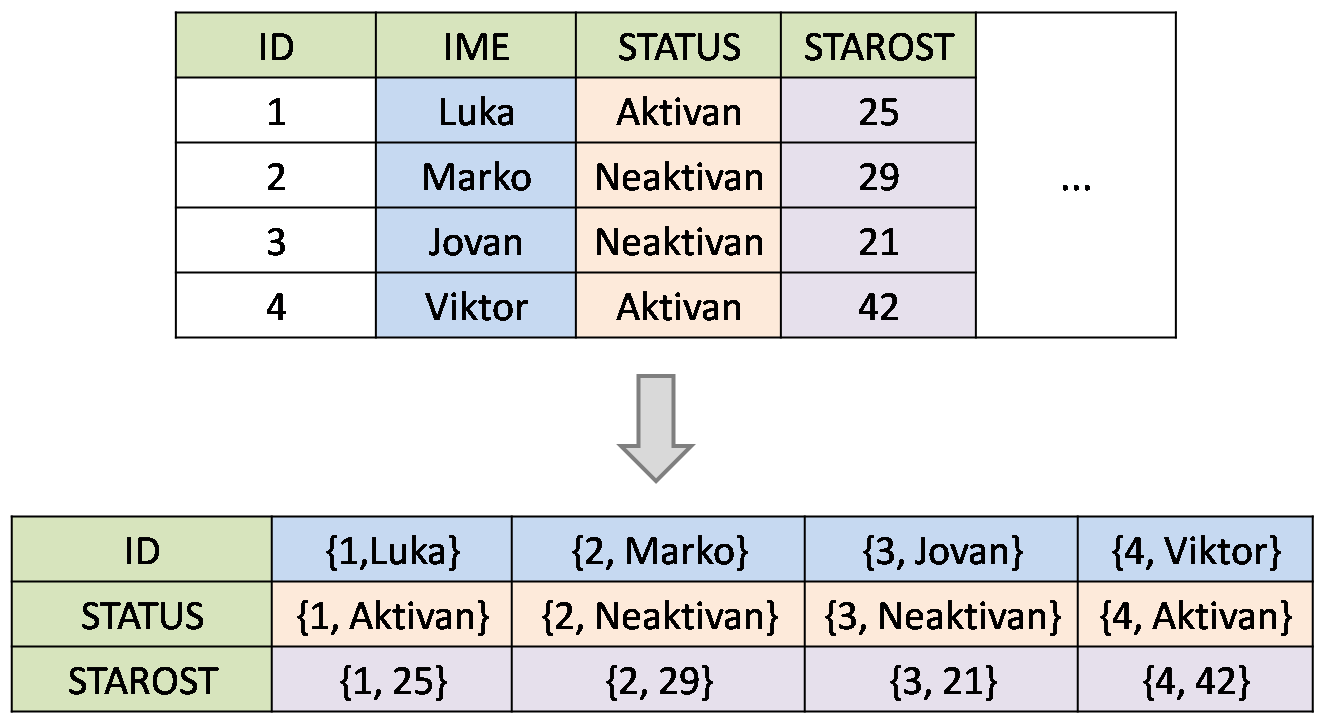
\includegraphics[width=0.9\textwidth]{relational-column-oriented.png}
  \caption{Kolonski orijentisan format}
  \label{fig:grafikon}
\end{figure}

% ------------------------------------------------------------------------------
\chapter{Modeli za upravljanje podacima}
\label{chp:razrada}
\section{Relacioni model}
\subsection{Opšte karakteristike}
Relacioni model je najpopularniji model za rad sa podacima. On podatke kao i veze izmedju njih predstavlja kroz skup relacija. Kao fundamentalna ideja iza relacionog modela stoji tabelarni prikaz podataka, sto uvecava njegovu intuitivnost. Da bi jedna tabela bila validna relacija u relacionom modelu ona mora ispunjavati sledeće uslove:

\begin{enumerate}
\item[\textbullet] Presek kolone i vrste jedinstveno određuje vrednosnu ćeliju.

\item[\textbullet] Sve vrednosne ćelije jedne kolone pripadaju nekom zajedničkom skupu. 

\item[\textbullet] Svaka kolona ima jedinstveno ime.

\item[\textbullet] Ne postoje dve identične vrste jedne tabele. 
\end{enumerate}

Iako ovakva formalizacija relacije deluje intuitivno (usled istorijskog uticaja koji je relacioni model ostavio na vizualizaciju organizacije podataka) ona je neophodna radi definisanja složenijih pojmova. 

\subsection{Koncept ključa relacionog modela}

Usled jedinstvenosti svake vrste relacije, jasno je da mora postojati skup kolona za koji važi da nikoja dva reda te relaciju nemaju identične vrednosti za svaku kolonu iz tog skupa. Takav skup se naziva \textit{superključ} relacije. Minimalan superključ naziva se \textit{ključ kandidat}. Svaka relacija može imati više ključeva kandidata, ali samo jedan od njih je  \textit{primarni ključ} koji mora imati definisanu vrednost za svaku njegovu kolonu.
\textit{Strani ključ} je kolona ili skup kolona čije vrednosti predstavljaju referencu na određeni red neke druge relacije. Primarni i strani ključ igraju veliku ulogu u očuvanju integriteta baze podataka o čemu ce biti reči u nastavku.

\subsection{Integritet relacionog modela}
Čuvanje integriteta relacionog modela predstavlja očuvanje vrednosti odnosno "istinitosti"  podataka koji se čuvaju u bazi. Ono nudi mehanizme očuvanja konzistentnosti podataka prilikom invazivnih operacija kao što su dodavanje reda, izmena reda ili brisanje reda u tabeli. Postoji vise vrsta integriteta u relacionom modelu: \textit{integritet entiteta}, \textit{integritet domena}, \textit{integritet neposojece vrednosti} i \textit{referencijalni integritet}.

 \textit{Integritet entiteta} kaže da svaka vrsta jedne relacije predstavlja jedan entitet i da kao takva ne može u okviru primarnog ključa, koji taj entitet identifikuje, imati nedefinisanu ili nepostojeću vrednost.

\textit{Integritet domena} nameće shemu po kojoj svaka kolona može uzimati vrednost iz unapred dodeljenih skupova vrednosti. 

\textit{Integritet nepostojece vrednosti} govori o eventulnim kolonama cije vrednosti ne mogu kao vrednost imatu nepostojecu vrednost kako se ne bi narušila uspostavljena biznis logika. 

\textit{Referencijalni integritet} nalaže da se svaki strani kljuc jedne tabele, ukoliko je definsan,  mora poklapati sa nekim od primarnih ključeva uparene relacije.

\subsection{Normalizacija}

Da bi se stanje u bazi očuvalo konzitentnim u relacionim modelima često se radi na izbegavanju \textit{redudantnosti} u podacima. Redudantni podaci zauzimaju višak prostora na disku i otežavaju kasnije održavanje sistema. Kako bi se izbegla redudantnost postoji jasno definisani postupci koji nam pomažu da organizujemo podatke tako da redudantnost umanjimo. Proces unapredđivanja logičkog dizajna baze tako da rešava problem redundantosti podataka, ali ne po cenu očuvanja integriteta, naziva se normalizacija. Teorija o normalizaciji se zasniva nad konceptima normalnih formi iz matematičke logike. U zavisnosti od toga koja pravila zadovoljava određena relacija, dodeljuje joj se normana forma. Trenutno postoji 5 defnisanih normalnih formi. 

\begin{enumerate}
\item Prva normalna forma (1NF)
	\begin{enumerate}
	\item[\textbullet] Svaka relacija mora imati primarni ključ koja jedinstveno određuje svaku vrste.
	\item[\textbullet] Svaka kolona mora saržati atomičnu (nedeljivu) vrednost.
	\item[\textbullet] Sve vrednosti jedne kolone pripadaju nekom zajedničkom skupu.
	\end{enumerate}

\item Druga normalna forma (2NF)
	\begin{enumerate}
	\item[\textbullet] Relacija mora biti 1NF
	\item[\textbullet] Sve vrednsti kolone koje ne pripadaju superključu relacije, direktno su određene celim primarnim ključem .
	\end{enumerate}

\item Treća normalna forma (3NF)
	\begin{enumerate}
	\item[\textbullet] Relacija mora biti 2NF
	\item[\textbullet] Nijedna kolona van ključa kandidata nije jedinstveno određena drugim kolonama koje ne pripadaju  ključu kandidatu.
	\end{enumerate}

\item Boyce-Codd normalna forma (BCNF)
	\begin{enumerate}
	\item[\textbullet] Relacija mora biti 3NF.
	\item[\textbullet] Svaka kolona koja ne pripada ključu mora biti jednistveno određena vrednostima superključa relacije.
	\end{enumerate}

\item Četvrta normalna forma (4NF)
	\begin{enumerate}
	\item[\textbullet] Relacija mora biti BCNF.
	\item[\textbullet] Regulisanje zavisnostni među kolonama tako da nema ponavljanja podataka.
	\end{enumerate}

\item Peta normalna forma (5NF)
	\begin{enumerate}
	\item[\textbullet] Relacija mora biti 4NF.
	\item[\textbullet] Reguliše zavisnosti između relacija tako da se izbegne potreba za komplikovanim upitima za dohvatanje podataka.
	\end{enumerate}

\end{enumerate}

\subsection{PostgreSQL}


PostgreSQL je objektno-relacioni sistem za upravljanje bazama podataka (ORDBMS) nastao kao potomak POSTGRES-a, proizvoda koji je nastao, a kasnije i razvijan na Berkliju, Univerzitet Kalifornija. PostgreSQL je otvorenog koda sa velikom SQL podrškom kao i modernim funkcionalnostima poput: kompleksnih upita, okidača, izmenjivih pogleda, transakcionog integriteta i mnogih drugih. Postgres nudi širok spektar proširenja od strane korisnika poput dodavanja novih tipova podataka, funkcija, operatora, agregagtnih funkcija itd. 

PostgresSQL koristi server-klijent model funkcionisanja. Sastoji se iz serverskog i klijentskog dela procesa. Serverski deo rukuje fajlovima baze podataka, prihvata konekcije, izvršava konkretne operacije nad bazom. Klijentski deo predstavlja aplikaciju kojom korisnik može da komunicira i rukuje podacima na serverskom delu. Klijent i server komunkciraju preko TCP/IP protokola. Serverski deo može raditi sa više konekcija istovremeno tako što svaka klijentska konekcija radi kao zaseban proces.

\section{Kolonski-orijentisani model}
% ------------------------------------------------------------------------------
\subsection{Opšte karakteristike}
\cite{ColumnarOriented}
Susret sa Big Data problemima dovelo je do potreba za tabelama koje imaju ogroman broj kolona, i ogroman broj redova u okviru tih tabela. Jasno je da nam je za potrebe različitih analitika potreban različit skup kolona. Navedena problematika predstavlja jedan od uočenih problema relacionih modela, gde je samo izvršavanje upita podrazumevalo dohvatanje svih kolona jednog reda, gde bi se filtriranje nepotrebnih kolona izvršavalo nakon što su se sve kolone učitale u memoriju. Kolonski orijentisan model dizajniran je tako da ovakav problem izbegne i uz to donese i druga poboljšanja o kojima će biti reči u nastavku.

Kolonski orijentisan model podatke tabele ne skladišti po redovima, već po kolonama. U prevodu, sve vrednosti kolone svih redova skladište se jedna do druge, a na konkretnu vrednosnu ćeliju referiše se pomoću ključa konkretnog reda kao i kolone čiju vrednost želimo da pročitamo. Ovakav dizajn doveo je do toga da za dohvatanje određenog skupa kolona nema potrebe da čitamo sve vrednosti tog sloga, već je dovoljno da znamo konkretan ključ tog reda kao i imena kolona čije vrednosti želimo da pročitamo.

S obzriom na bliskost   podataka na disku, nameće se mogućnost kompresije podataka, a s obzirom da su ti slični podaci lokalizovani na disku nema potrebe za velikom količinom meta informacija o kompresiji, što ovaj model čini posebno pogodnim za njihovu primenu.

Kolonski orijentisan model kao i većina ostalih nerelacionih modela, nudi fleksibilnost sheme. To kao posledicu to da eventualna promena strukture podataka nece bitno uticati na unapred definisanu shemu, kao ni iziskivati migraciju podataka, kao sto bi to bio slucaj kod relacionog modela. Osim toga fleksibilnost sheme se ogleda i u tome sto je broj kolona jednog vektora neogranicen, sto daje dosta prostora za eksperimentisanje sa dizajnom baze. Primer toga kako ovakvo svojstvo modela može doprineti dostizanju prednosti pri analitičkom sistemu možete videti na slici SLIKA 1. 

\subsection{Popularni primenjivi algoritmi kompresije}
\cite{ColumnarOptimizations}
\subsubsection{Enkodiranje zasnovano na recniku}

Enkodiranje zasnovano na rečniku (Dictionary based encoding) jeste tehnika kompresije podataka koja se može primeniti na vrednosti jedne kolone. Najefikasnija je nad kolonama koje imaju mali skup mogućih vrednosti. Rade tako što se u memoriji sačuvaju sve moguće vrednosti te kolone i svakoj od njih se dodeli ključ. Veličina ključa je direktno zavisna od kardinalnosti skupa vrednosti te kolone. Svaki unos ili izemna vrednosti kolone u konsultaciji sa postojećim rečnikom radi enkodiranje pristigle vrednosti, a svako dohvatanje vrednosti radi dekodiranje sačuvane vrednosti. Ovim se izbegava smanjuje ponavljanje velikih podataka tako smanjujući potrebnu memoriju na disku. Uglavnom su pogodne primene nad kolonama sa statičkim i opisnim podacima koji se ponavljaju.
\begin{figure}[!ht]
  \centering
  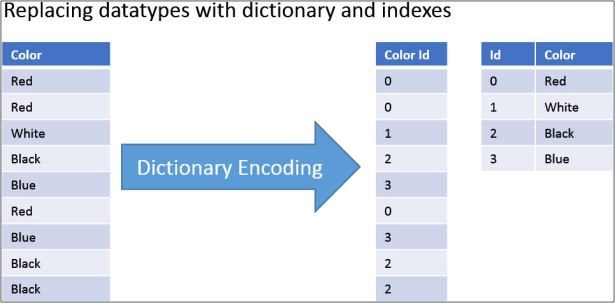
\includegraphics[width=0.6\textwidth]{DictionaryEncoding.jpg}
  \caption{Enkodiranje zasnovano na recniku}
  \label{fig:grafikon}
\end{figure}


\subsubsection{Enkodiranje po broju ponavljanja}

Enkodiranje po broju ponavljanja (Run Length Encoding) je jednostavan mehanizam za kompresiju podataka pogodan za kolonski orijentisane baze podataka. Funkcioniše tako što kada se naiđe na vrednost koja se ponavlja, ne skladišti duplikate već sačuva tu vrednost jednom a dodatno kao meta informaciju prosledi koliko se ta vrednost ponavlja. Takav vid optimizacije najkorisnije je očigledno kada su vrednosti sortirane, a s obzirom da su vrednosti kolona u kolonski orijentisanim bazama jedna do druge to otvara prostor za ovaj vid kompresije podataka kako bi se umanjilo zauzeće prostora.

\begin{figure}[!ht]
  \centering
  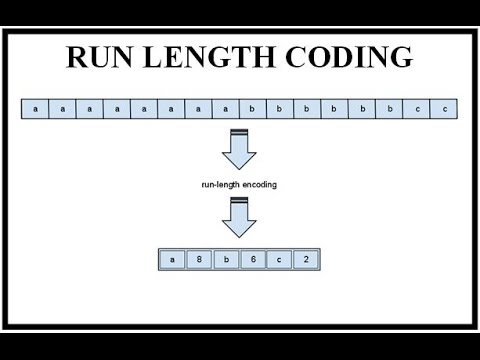
\includegraphics[width=0.6\textwidth]{run-length-encoding.jpg}
  \caption{Enkodiranje po broju ponavljanja}
  \label{fig:grafikon}
\end{figure}

\subsubsection{Delta enkoding}
Delta enkoding je mehanizam za optimizaciju prostora baze podataka koji se zasniva na čuvanju razlike između objekata a ne celih vrednosti. Primera za upotrebu ima dosta a jedan od najčešćih je slučaj datumskih kolona, gde će nam referentna vrednost biti neki konkretan datum, a vrednosti ostalih kolona će biti čuvane kao razlika u odnosu na njega, te je očigledna velika količina prostora koja se čuva u takvom slučaju korišćenjem ovog vida optimizacije.

\begin{figure}[!ht]
  \centering
  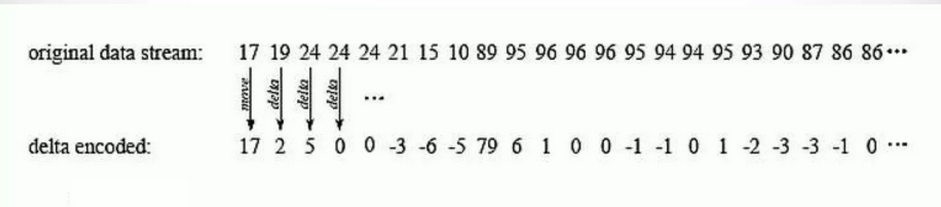
\includegraphics[width=0.9\textwidth]{delta-encoding.png}
  \caption{Delta enkoding}
  \label{fig:grafikon}
\end{figure}

\subsection{HBase}

HBase je distribuirana kolonski orijentisana nerelaciona baza podataka  pisana u javi. Izvršava se nad HDFS (Hadoop Distributed File System) arhitekturom. Nastala je 2007 kao prototip BigTable baze koja je modelovana u okviru Google-ovog članka 2006 \cite{BigTable}. 

Arhitektura HBase klastera sastoji se iz tri glavne komponente: HMaster, Region server, i HDFS.  Ove komponente je najbolje opisati kroz interfejse koje oni implementiraju. 

HDFS je sloj nad kojim radi HBase arhitektura. Osnovna organizaciona jedinica podataka koju HBase upisuje na HDFS jeste HFile. HFile može biti podeljen na više blokova u okviru HDFS-a ali o tome se on ne brine. 

Region server implementira HRegionRegionInterface, odnosno implementira servise koji se bave operacijama nad podacima i održavanjem i upravljanjem regiona. Jedan Region sadrži određeni skup podataka za neke ključeve koji su u određenom rasponu vrednosti.  Njega možemo zamisliti kao indeks za dohvatanje HFile-ova sa HDFS-a.  Svaka izmena koja treba da se izvrši na disku prvo se upisuje u WAL (Write ahead log), a nova izmenjena vrednost se upisuje u MemStore fajl. Kada se MemStore fajl upuni tek tada se izmene flush-uju u jedan HFile koji dalje ide na HDFS. 

HMaster implementira HMasterInterface koji sadrži servise koji rade sa metainformacijama o tabelama, familijama kolona, kao i regiona. Uloga Mastera je da za svaki konkretan row id može da odredi koji region odnostno region server treba da bude pročitan kako bi se izvršila odgovarajuća operacija. Za postizanje navedene funkcionalnosti HMaster koristi Zookeeper \cite{BigTable} servis. Pored toga master servis ima pozadinske procese koji regulišu rad load balansera i sadržaj hbase:meta tabele.

\begin{figure}[!ht]
  \centering
  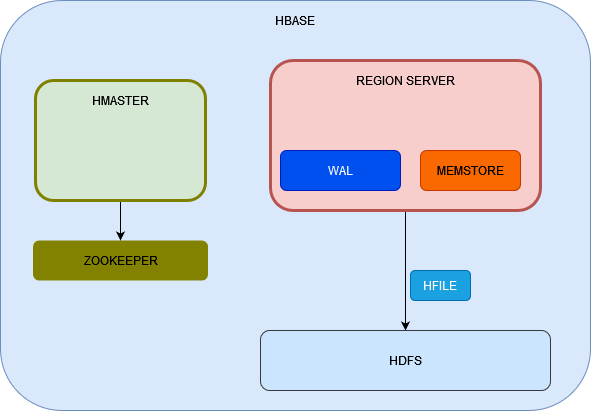
\includegraphics[width=0.7\textwidth]{hbase-arhitektura.png}
  \caption{HBase arhitektura}
  \label{fig:grafikon}
\end{figure}

\pagebreak

\section{Glavne razlike između relacionog i kolonski-orijentisanog modela}

\subsection{ACID vs BASE}

ACID (Atomicity, Consistency, Isolation, Durability) svojstva služe kao garancija tačnosti i konzistetnosti podataka prilikom konkurentnom pristupu. 

Atomicity se može objasniti pravilom: Jedna transakcija se izvršava u celini ili se ne izvršava nijedan njen deo. U prevodu, dejstvo transakcije je nedeljivo. 

Durability garantuje da će kompletirana transakcija u slučaju prekida rada sistema pre nego što su izmene reflektovane na disk, biti upamćena i izvršena nakon restarta sistema. Svaka izmena se upisjue u log fajl pre nego što je reflektovana na disk, kako bi se operacije mogle poništiti u slučaju poništavanja transakcije.

Consistency se čuva od strane korisnika. Bitno je da korisnik koji pokreće transakciju vodi računa o tome da stanje podataka ostane u konzistentom stanju.

Isolation svojstvo nalaže da se transakcije međusobno izolovane tako da izvršavanje jedne transakcije ne može uticati na izvršavanje druge. Ovo se obezbeđuje pomoću scheduler-a od strane samog sistema za upravljanje bazom podataka.

BASE (Basic Availability, Soft state, Eventual consistency) je skup svojstava koje je definisao Eric Brewer , a koja su nastala usled zelje da se formalizuju svojstva koja u Big Data svetu garantuju da je baza pogodna za horizontalno skaliranje a ujedno daje vid konzistentnosti koji je neophodan. 

Basically available  svojstvo kaze da ukoliko imamo klaster sa vise pojedicanih node-ova baze, problem sa jednim od njih nece spreciti da ostali node-ovi procesiraju zahteve i salju odgovore.

Soft state -  svojstvo kaze da se stanje podataka moze menjati, cak i u trenucima kada nema spoljnih komunikacija sa bazom podataka. Ovo je posledica treceg svojstva.

Eventual consistency garantuje da ce baza podataka u periodima kada nema spoljne komunikacije sa klijentima, postati konzistentna kroz neki vremenski period. 

Kolonski orijentisan model nacelno ne mora da ispunjava BASE svojstva, ali to obicno jeste slucaj upravo zbog horizontalnog skaliranja koja ima tendenciju da ponudi.


\subsection{Skalabilnost}

\begin{figure}[!ht]
  \centering
  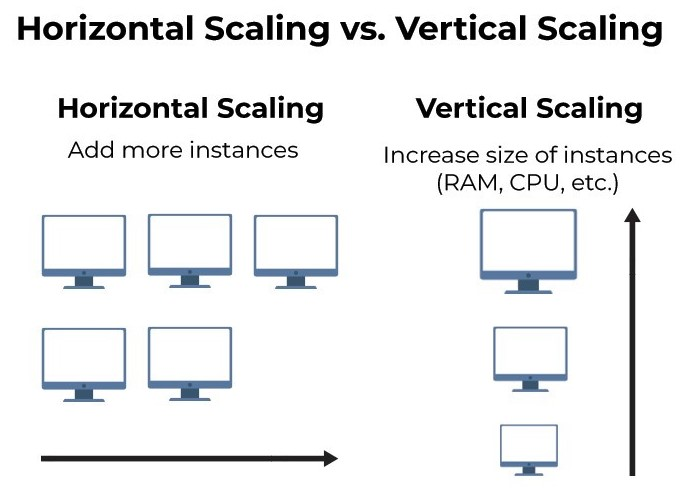
\includegraphics[width=0.6\textwidth]{horizontal-vertical-scaling.jpg}
  \caption{Enkodiranje po broju ponavljanja}
  \label{fig:grafikon}
\end{figure}

% ------------------------------------------------------------------------------
\chapter{Slučajevi upotrebe}
% ------------------------------------------------------------------------------
\section{Opis i sadržaj eksperimenta}
Analiza i uporedjivanje slucajeva upotrebe bice realizovani na osnovu teorijskih i prakticnih  izvora i istrazivanja. Svaki primer ce biti pracen eksperimentom koji ce se sastojati od izvrsavanja razlicitih vrsta postupaka. Kao platforma za realizaciju eksperimenata koriscen je host sa docker engine-om. Specifikacije Host-a data je na slici. Pokretanje svakog od eksperimenata je identicno. U okviru repozitorijuma nalazi se sav shell i java kod kao i uputstvo za pokretanje svakog od eksperimenta, zajedno sa deplojment dijagramom.

Svakom eksperimentu dodeljen je precizno definisan kontekst radi uspostavljanja potpune kontrole okruzenja u kojem se eksperiment realizuje. U svrhu definisanja konteksta eksperimenata delom su iskoriscene poznate specifikacije za benchmark bazi podataka. Konkretno za slucaj OLTP okruzenja konsultovana je TPC-C specifikacija, za slucaj OLAP okruzenja konsultovana je TPC-H specifikacija. Distribuirao okruzenje je izuzeto.

Analiza rezultata eksperimenta sprovodi se kroz vise faza. Prva faza je uporedjivanje slozenosti , sto arhitekturalne, sto shematske, realizacije konkretnog slucaja upotrebe kao i da li je konkretan slucaj upotrebe moguce realizovati sa postojecom tehnologijom. Druga faza je uporedjivanje efikasnosti, koja podrazumeva uporedjivanje vremena izvrsavanja programa.  Svaka od faza ce ukljucivati tekstualnu diskusiju, slike kao i druge graficke prikaze ukoliko su pogodni.

Kako bi se postigao dovoljan dokaz koncepta (eng. proof of concept), ali i doslednost modernom
vremenu, kategorije slucajeva upotrebe koji ce biti obuhvaceni su:
\begin{enumerate}
\item Onlajn transakciono procesiranje (OLTP)
\item Onlajn analiticko procesiranje (OLAP)
\item Primena u distribuiranom okruzenju
\end{enumerate}

\subsection{Platforma testiranja}

Kao okruženje za izvršavanje eksperimenata korišćen je docker.  Oba predstavnika bice pokrenuta u okviru nezavisnih kontejnera na jednom host-u sa docker engine-om. Svaki test predstavlja jedan java program koji se izvršava na konkretnom kontejneru, kako bi se izbegao bilo kakav vid spoljne komunikacije i kako bi se stekla što preciznija slika na osnovu rezultata merenja.  

Svaki test imaće određene parametrke koji se postavljaju pri pokretanju testa. Parametri su broj iteracija/transakcija koje će test izvršiti kao i broj konekcija(odnosno klijenata) koji će paralelno u zasebnim nitima obavljati svoj deo posla.

Programi za OLAP i OLTP testiranje kreiraju se nezavisno s obzirom na kontekst (drugačiji model i test logika) u kojem se izvršavaju. Za OLTP i OLAP testiranje postoji po jedan maven artifakt kojeg će koristiti i HBase i Postgres jar-ovi koji predstavljaju kostur programa za testiranje. Svrha tog zajedničkog jar-a jeste da garantuje da će oba testa imati isti kostur, te da će se HBase i Postgres testovi razlikovati jedino po implementaciji  odgovarajućih utility funkcija. 


S obzirom da je u OLAP testu obuhvaćen segment za merenje bulk load-a podataka iz odgovarajućih csv fajlova, taj segment je takođe uključen u kostur testiranja.

Napomena: Kako su za predstavnike izabrani PostgresSQL i HBase,  za rezultate merenja u nastavke treba uzeti u obzir da implementacija navedenih koncepata nije opsta za sve Relacione sisteme kao ni za sve kolonski orijentisane baze podataka.


\lstset{
  basicstyle=\footnotesize,
  keywordstyle=\color{red},
  backgroundcolor = \color{lightgray},
  numbers=left,
  showstringspaces=false,
  frame=single
}

\begin{lstlisting}[title={docker-compose.yml},captionpos=t]
services: 
  postgres:
    container_name: postgres
    ports:
      - "5433:5432"
    environment:
      - POSTGRES_PASSWORD=postgres
      - POSTGRES_USER=postgres
      - POSTGRES_DB=postgresdb
    build:
      context: .
      dockerfile: ./Dockerfile_postgres
  hbase-master:
    image: blueskyareahm/hbase-base:2.1.3
    command: master
    ports:
      - 16000:16000
      - 16010:16010
    volumes:

  hbase-regionserver:
    image: blueskyareahm/hbase-base:2.1.3
    command: regionserver
    ports:
      - 16030:16030
      - 16201:16201
      - 16301:16301

  zookeeper:
    image: blueskyareahm/hbase-zookeeper:3.4.13
    ports:
      - 2181:2181
\end{lstlisting}


\lstset{
  language=Java,
  basicstyle=\footnotesize,
  keywordstyle=\color{red},
  backgroundcolor = \color{lightgray}
}

\begin{lstlisting}[title={OLTPBenchmarkExecutor.java},captionpos=t]
default void executeOLTPWorkload
    (BenchmarkUtility util, BenchmarkOLTPUtility oltpUtil, 
     int transNum, int clNum)  {

        List<Integer> transPerClientList = new ArrayList<>();
        int transactionsToAssign = totalTransactions;
        int transactionsPerClient = transactionsToAssign / clNum;

        for(int i = 0; i<clNum;i++){
            transPerClientList.add(transactionsPerClient);
            transactionsToAssign-=transactionsPerClient;
        }
        if (transactionsToAssign > 0) {
            int transactionForLastClient = transPerClientList.get(
							clNum - 1);
            transPerClientList.set(clNum - 1, 
			transactionForLastClient + transactionsToAssign
					  );
        }

        assert clNum==transPerClientList.size();

        Thread[] threads = new Thread[clNum];
        CountDownLatch latch = new CountDownLatch(numOfClients);
        for(int i = 0;i<clNum;i++){
            threads[i] = new Thread(
				new BenchmarkSingleClientExecutor(
					util,oltpUtil,
					i*transPerClientList.get(i),
					transPerClientList.get(i),
					latch)
			  );
        }


        long startTimestamp = System.currentTimeMillis();
        for(int i = 0;i<clNum;i++){
            threads[i].start();
        }
        latch.await();
        long endTimestamp = System.currentTimeMillis();
        System.err.println("Total benchmark duration: " + 
		(endTimestamp-startTimestamp));
    }
\end{lstlisting}

\lstset{
  language=Java,
  basicstyle=\footnotesize,
  keywordstyle=\color{red}
}

\begin{lstlisting}[title={OLAPBenchmarkExecutor.java},captionpos=t]
default void executeBulkLoad
	(BenchmarkUtility util,BenchmarkOLAPUtility olapUtil) {
        long bulkLoadStart = System.currentTimeMillis();
        olapUtility.bulkLoad(benchmarkUtility.connect());
        long bulkLoadEnd = System.currentTimeMillis();
        System.out.println("Bulk load duration: "+
       	 	 (bulkLoadEnd-bulkLoadStart));
    }

default void executeOLAPWorkload
    (BenchmarkUtility util, BenchmarkOLAPUtility olapUtil, 
          int iterNum, int clNum)  {

        List<Integer> itsPerClientList = new ArrayList<>();
        int iterationsToAssign = iterNum;
        int iterationsPerClient = iterationsToAssign / clNum;

        for(int i = 0; i<clNum;i++){
            itsPerClientList.add(iterationsPerClient);
            iterationsToAssign-=iterationsPerClient;
        }
        if (iterationsToAssign > 0) {
            int iterationsForLastClient = itsPerClientList.get(
							clNum - 1);
            itsPerClientList.set(clNum - 1, 
			iterationsForLastClient + iterationsToAssign
					  );
        }

        assert clNum==itsPerClientList.size();

        Thread[] threads = new Thread[clNum];
        CountDownLatch latch = new CountDownLatch(clNum);
        for(int i = 0;i<clNum;i++){
            threads[i] = new Thread(
				new BenchmarkSingleClientExecutor(
					util,olapUtil,
					i*itsPerClientList.get(i),
					itsPerClientList.get(i),
					latch)
			  );
        }


        long startTimestamp = System.currentTimeMillis();
        for(int i = 0;i<clNum;i++){
            threads[i].start();
        }
        latch.await();
        long endTimestamp = System.currentTimeMillis();
        System.err.println("Total benchmark duration: " + 
		(endTimestamp-startTimestamp));
    }
\end{lstlisting}

\subsection{Priprema okruženja}

Priprema okruženja za sprovođenje eksperimenata podrazumeva build-ovanje  .jar fajlova za testiranje, pokretanje docker kontejnera , prebacivanje svih neophodnih resursa vezanih za kreiranje modela baze podataka i eventualnih resursa za bulk load vrednosti u tabele na odgovoarajuće docker kontejnere.


\lstset{
  language=bash,
  basicstyle=\footnotesize,
  keywordstyle=\color{red}
}

\begin{lstlisting}[title={prepareEnv.sh},captionpos=t]
#!/bin/bash
echo 'PREPARING ENVIRONMENT...';

rm -f ./hbase_setup_model.jar
rm -f ./benchmark_hbase.jar
rm -f ./benchmark_postgres.jar

export JAVA_HOME="$JAVA_8";
mvn -f ./hbase_setup_model clean compile assembly:single;
mvn -f ./benchmark_hbase clean compile assembly:single;

export JAVA_HOME="$JAVA_17";
mvn -f ./benchmark_postgres clean compile assembly:single;


docker-compose -f docker-compose.yml up --build -d;
docker exec -it hbase-master-1 sh -c "java -jar hbase_setup_model.jar";




\end{lstlisting}

\begin{figure}[!ht]
  \centering
  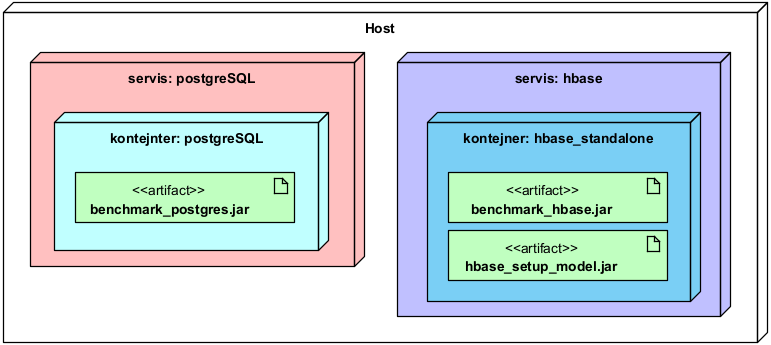
\includegraphics[width=0.9\textwidth]{deployment_diagram.png}
  \caption{Enkodiranje po broju ponavljanja}
  \label{fig:grafikon}
\end{figure}

\pagebreak

\section{Primena u online transakcionom procesiranju (OLTP)}

Online transakciono procesiranje obuhvata kratke, jednostavne, uchestale promene  na relativno malom skupu podataka. Primer koji cemo koristiti jeste uopstena transakcija korisnika gde sa jednog racuna treba da se prebaci novac na drugi racun.

Specifikacija PostgresSQL modela:

Specifikacija HBASE modela:

Rezultati:

\section{Primena u online analitičkom procesiranju (OLAP)}

OLAP procesiranje sacinjeno je od skoro iskljucivo citanja podataka. Upiti koji se koriste obicno imaju parametre, imaju visok nivo kompleksnosti i visok procenat podataka kojima pristupa.
Primer koji cemo koristiti jeste uopsten primer odrzavanja trgovinskog lanca koji ima skup musterija, proizvoda, dobavljaca,  narudzbina. 
Nas OLAP eksperiment ce se sastojati iz dohvatanja izvestaja o ukupnom kvanitetu, ceni nakon odbijanja poreza, prosecnom popustu za dati status stavke narudzbine.


Specifikacija Postgres modela:

Specifikacija HBASE modela:

Rezultati:

\section{Primena u distribuiranom okruženju}
\subsection{Skalabilnost}
\subsubsection{Vertikalna skalabilnost}
\subsubsection{Horizontalna skalabilnost}
\subsection{CAP teorema}

\chapter{Zaključak}

% ------------------------------------------------------------------------------
% Literatura
% ------------------------------------------------------------------------------
\literatura

% ==============================================================================
% Završni deo teze i prilozi
\backmatter
% ==============================================================================

% ------------------------------------------------------------------------------
% Biografija kandidata
\begin{biografija}
\textbf{Вук Стефановић Караџић} (\emph{Тршић, 26. октобар/6. новембар
  1787. — Беч, 7. фебруар 1864.}) био је српски филолог, реформатор
српског језика, сакупљач народних умотворина и писац првог речника
српског језика.  Вук је најзначајнија личност српске књижевности прве
половине XIX века. Стекао је и неколико почасних доктората.
Учествовао је у Првом српском устанку као писар и чиновник у
Неготинској крајини, а након слома устанка преселио се у Беч,
1813. године. Ту је упознао Јернеја Копитара, цензора словенских
књига, на чији је подстицај кренуо у прикупљање српских народних
песама, реформу ћирилице и борбу за увођење народног језика у српску
књижевност. Вуковим реформама у српски језик је уведен фонетски
правопис, а српски језик је потиснуо славеносрпски језик који је у то
време био језик образованих људи. Тако се као најважније године Вукове
реформе истичу 1818., 1836., 1839., 1847. и 1852.
\end{biografija}
% ------------------------------------------------------------------------------

\end{document} 